% ====chapter=====
\myChapter{Approche proposée pour la génération d'applications web pilotées par BPMN}{Approche proposée}
\label{chap:approche-prooweb}
\myMiniToc{mysection}{Sommaire}

\mySection{Introduction}{}

Ce chapitre présente l'approche d'ingénierie proposée dans ce mémoire. Il montre comment ProOWeb exploite un modèle BPMN, complété par une spécification applicative, pour générer une application web complète et fonctionnelle. L'objectif est de passer d'un processus métier modélisé à un projet logiciel exécutable, composé d'un front-end, d'un back-end, d'une persistance, d'un runtime de processus, de règles de sécurité et de mécanismes de déploiement.

Après l'état de l'art, le problème à résoudre est maintenant précis : conserver le lien entre le processus métier et le code produit, tout en laissant au développeur la possibilité de faire évoluer l'application générée. Pour cela, ProOWeb s'appuie sur une démarche proche de l'ingénierie dirigée par les modèles : le BPMN décrit le workflow, la spécification \textit{spec-v1} décrit les informations applicatives manquantes, puis un modèle pivot prépare la génération des artefacts logiciels \cite{omg2014mda,omg2013bpmn}.

La suite du chapitre est organisée comme suit. La section \ref{sec:chap3-vue-ensemble} donne la vue d'ensemble de l'approche. La section \ref{sec:chap3-architecture} présente les différentes parties de l'architecture ProOWeb. La section \ref{sec:chap3-spec} décrit la spécification \textit{spec-v1}. La section \ref{sec:chap3-transformations} expose les règles de transformation et de génération. Enfin, la section \ref{sec:chap3-preservation} présente les mécanismes prévus pour préserver le code personnalisé lors des régénérations.
\mySection{Vue d'ensemble de l'approche}{}
\label{sec:chap3-vue-ensemble}

\subsection{Problème traité et principe général}

L'approche proposée vise à générer une application web complète et fonctionnelle à partir d'un processus métier modélisé. Dans ce travail, une application complète ne désigne pas une simple collection de fichiers. Elle correspond à un projet logiciel structuré, comprenant un front-end, un back-end, une persistance, des règles de sécurité, un runtime de processus, des vues de traitement, des fonctions de supervision, des profils d'exécution et des scripts nécessaires au déploiement. ProOWeb doit donc produire un socle applicatif que le développeur peut exécuter, versionner, tester, adapter et faire évoluer.

Le choix de BPMN comme modèle d'entrée est justifié par sa place dans la modélisation des processus métier. BPMN 2.0 fournit une notation standard pour représenter les activités, événements, passerelles et flux de séquence d'un processus \cite{omg2013bpmn}. Dans le domaine du Business Process Management, un processus n'est pas seulement une succession d'étapes ; il organise le travail entre acteurs, systèmes, règles et informations \cite{dumas2018fundamentals,weske2012bpm}. Cependant, BPMN ne décrit pas toujours les détails nécessaires à une application web : champs de formulaires, règles de visibilité, structures de persistance, droits d'accès ou stratégies d'affectation.

ProOWeb repose donc sur un double modèle d'entrée. Le premier modèle est le fichier BPMN, qui conserve la responsabilité de représenter le déroulement du processus. Le second est la spécification \textit{spec-v1}, qui apporte les informations applicatives nécessaires à la génération. Cette séparation évite de surcharger le diagramme BPMN avec des détails techniques, tout en empêchant l'application générée de s'éloigner du processus métier.

Le principe général peut être résumé en quatre étapes. D'abord, ProOWeb analyse le modèle BPMN et extrait les éléments utiles au workflow. Ensuite, il lit la spécification \textit{spec-v1} et associe les informations applicatives aux activités concernées. Puis, il construit un modèle applicatif intermédiaire qui stabilise les contrats de génération. Enfin, il produit les artefacts front-end, back-end, persistance, configuration et déploiement à partir de ce modèle intermédiaire.

\subsection{Positionnement dans le cycle MDA}

La Model-Driven Architecture fournit un cadre pertinent pour comprendre la progression proposée. Dans cette approche, le développement repose sur des modèles qui se rapprochent progressivement de l'implémentation : modèle indépendant du calcul, modèle indépendant de la plateforme, modèle spécifique à la plateforme et code \cite{omg2014mda,mellor2003mda}. ProOWeb ne reprend pas ce cadre comme une classification abstraite ; il l'utilise pour clarifier les responsabilités de chaque niveau de la chaîne de génération.

Au niveau PIM, le processus est décrit sans dépendance directe à Spring Boot, React, Liquibase ou à une technologie de déploiement. Le BPMN représente le comportement métier, tandis que \textit{spec-v1} complète la conception applicative sans encore imposer la forme exacte des classes Java ou des composants React. La spécification reste donc proche des préoccupations métier et applicatives : qui peut démarrer une instance, qui peut traiter une tâche, quelles données sont consultées, quelles sorties sont produites et quels rôles peuvent voir les informations.

Au niveau PSM, ProOWeb construit des contrats intermédiaires : \textit{runtime contract}, \textit{data contract}, catalogues front-end, catalogues de formulaires et registres de processus. Ces contrats sont plus proches de l'application cible. Ils indiquent les transitions, les rôles, les stratégies d'affectation, les sources de données, les mappings de sortie et les éléments à exposer au front-end. Ils ne sont pas encore du code source, mais ils rendent les informations suffisamment précises pour que les gabarits puissent produire des artefacts cohérents.

Au niveau code, les transformations modèle-à-texte matérialisent les décisions précédentes. Une activité manuelle devient une tâche accessible dans l'interface, une route back-end, une règle d'autorisation et une transition de runtime. Une donnée partagée devient une entité persistante, un repository, un changement de schéma et un champ exploitable par les formulaires. Une règle de visibilité devient un filtrage côté API et une adaptation côté interface.

\begin{table}[H]
\centering
\small
\caption{Positionnement de ProOWeb dans le cycle MDA}
\label{tab:chap3-positionnement-mda}
\begin{tabular}{p{3.2cm}p{5.2cm}p{5.4cm}}
\hline
\textbf{Niveau} & \textbf{Contenu dans ProOWeb} & \textbf{Rôle dans la génération} \\
\hline
PIM & BPMN et spécification \textit{spec-v1} & Décrire le workflow, les rôles, les entrées, les sorties, la visibilité et les données sans dépendre directement du code cible. \\
PSM & Contrats intermédiaires, catalogues et registres & Stabiliser les informations dans une forme exploitable par les générateurs front-end, back-end et persistance. \\
Code & Projet Spring Boot, React/Vite, persistance, configuration et scripts & Produire une application web complète, exécutable, versionnable et personnalisable. \\
\hline
\end{tabular}
\end{table}

Ce positionnement permet de réduire un risque classique des générateurs : concentrer trop de logique dans les templates. Dans ProOWeb, les gabarits ne doivent pas deviner les règles métier. Ils traduisent des décisions déjà validées dans le modèle pivot. Cette séparation améliore la traçabilité et facilite les tests de la chaîne de génération.

\subsection{Contribution méthodologique de l'approche}

La contribution de ProOWeb se situe à l'intersection de trois préoccupations. La première est la modélisation du processus. Le BPMN reste la référence du workflow et permet de maintenir une continuité avec les pratiques de modélisation métier. La deuxième est la génération d'une application web complète. Le framework ne se limite pas à produire des écrans ou des API isolées ; il organise un projet cible avec ses modules fonctionnels et techniques. La troisième est la maintenance du code généré. La régénération est traitée comme une opération contrôlée, accompagnée par un manifeste, des sauvegardes, des rapports et des mécanismes d'extension.

Cette contribution se distingue ainsi des approches qui génèrent uniquement des prototypes d'interface \cite{diaz2018,sajji2023}, des API pour moteurs de workflow \cite{pietruck2020} ou des applications fortement liées à une plateforme d'exécution particulière \cite{schaffer2021,neto2022}. ProOWeb vise un résultat plus directement exploitable par une équipe de développement : une application web générée, mais ouverte à l'adaptation.

\mySection{Architecture globale du framework proposé}{}
\label{sec:chap3-architecture}

L'architecture de ProOWeb est organisée autour de quatre parties complémentaires. La première regroupe les modèles d'entrée. La deuxième correspond au noyau de génération du framework. La troisième représente l'application web produite. La quatrième concerne l'exploitation et l'évolution de cette application. Cette lecture par blocs permet de distinguer clairement ce qui est fourni par le concepteur, ce qui est traité par ProOWeb, ce qui est généré et ce qui est utilisé ensuite par les acteurs du système.

\begin{figure}[H]
\centering
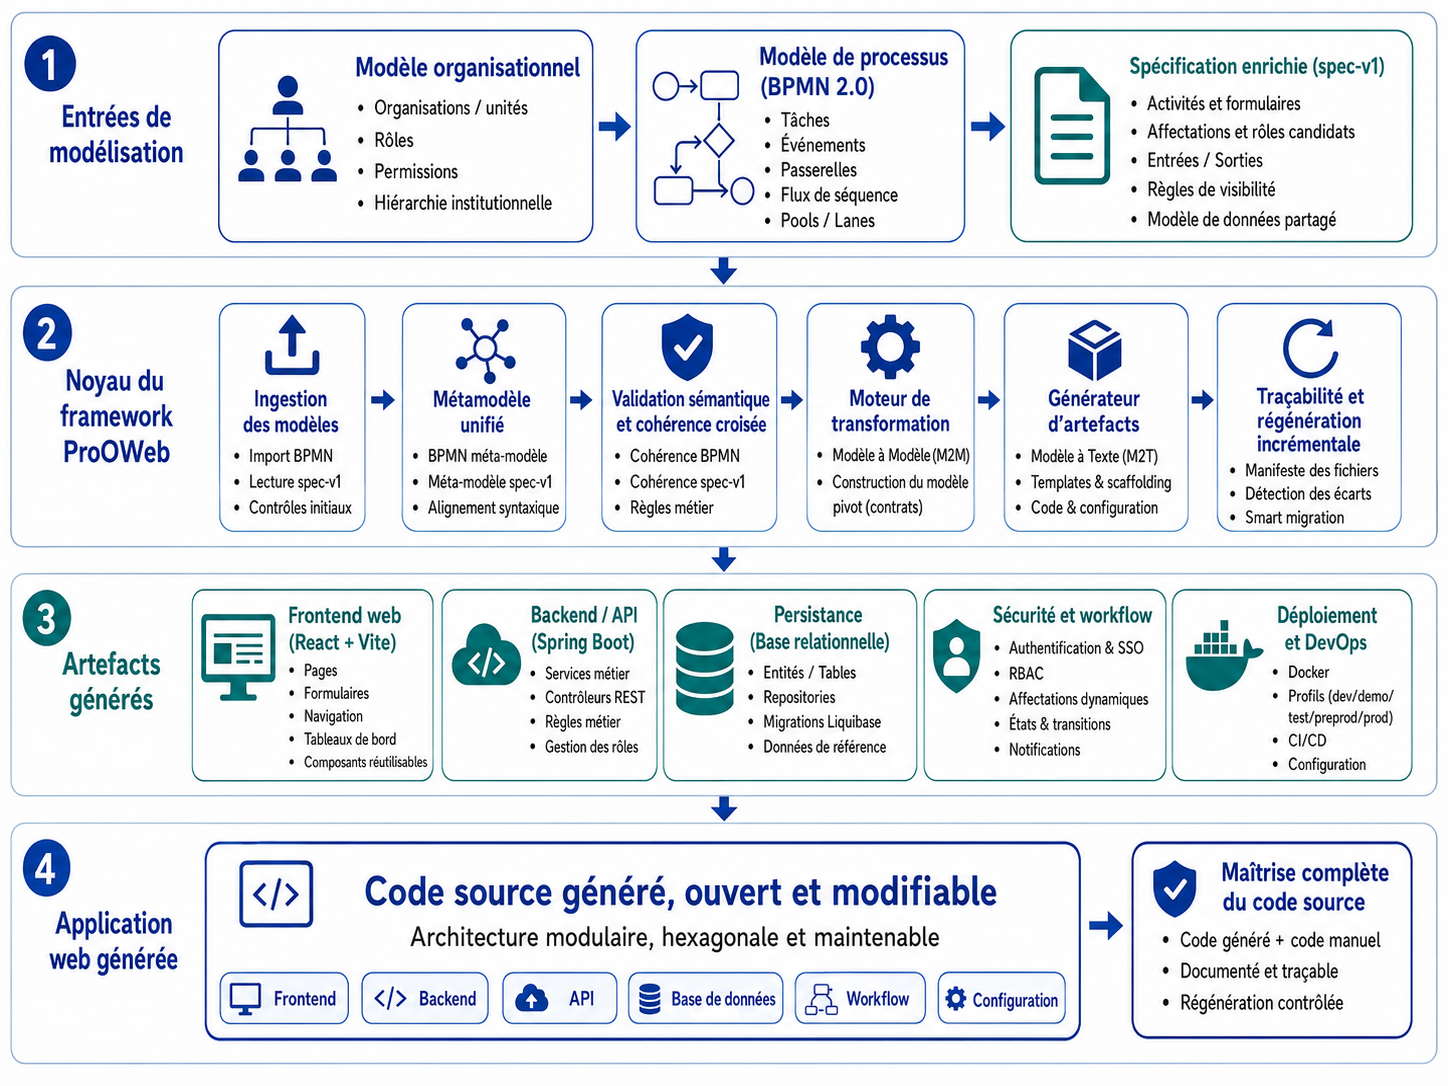
\includegraphics[width=0.82\textwidth]{Chap3/images/architecture_ProOWeb1.png}
\caption{Architecture générale de ProOWeb}
\label{fig:chap3-architecture-prooweb}
\end{figure}

\subsection{Modèles d'entrée de ProOWeb}

Le premier bloc de l'architecture regroupe les éléments à partir desquels la génération est lancée. Il comprend principalement le modèle BPMN, la spécification \textit{spec-v1}, les informations organisationnelles et la configuration du projet cible. Ce bloc correspond à la partie métier et applicative de l'approche.

Le modèle BPMN décrit le déroulement du processus. Il précise les activités, les événements, les passerelles et les flux de séquence. Il constitue donc la base du workflow. Cependant, il ne contient pas toutes les informations nécessaires à la génération d'une application web. Pour cette raison, ProOWeb lui associe une spécification \textit{spec-v1}. Cette spécification complète le processus avec les rôles, les règles d'affectation, les données d'entrée, les sorties, les stratégies de stockage et les règles de visibilité.

Les informations organisationnelles permettent de relier les tâches aux acteurs de l'application. Elles indiquent notamment les rôles disponibles, les profils qui peuvent démarrer ou superviser un processus et les responsabilités associées aux activités. La configuration du projet cible précise enfin certains choix techniques : nom du projet, modules à produire, profils d'exécution, activation de la persistance, génération du front-end ou du back-end, et options de déploiement.

Ce premier bloc joue donc le rôle de source de vérité. ProOWeb ne doit pas inventer les informations métier. Il doit les lire, les valider et les transformer. Cette exigence limite les interprétations implicites et facilite la traçabilité entre le modèle de départ et le code produit.

\subsection{Noyau de génération du framework}

Le deuxième bloc correspond au coeur de ProOWeb. Il prend en entrée les modèles précédents et les transforme progressivement en artefacts générables. Ce noyau comprend l'ingestion BPMN, l'enrichissement par la spécification, la validation croisée, la construction du modèle pivot, les transformations modèle-à-modèle, les transformations modèle-à-texte et la traçabilité des fichiers générés.

L'ingestion BPMN extrait les éléments utiles du diagramme : activités, événements, flux, passerelles, liens entrants et liens sortants. Cette étape permet de reconstruire une représentation exploitable du workflow. L'enrichissement associe ensuite chaque activité BPMN aux informations déclarées dans \textit{spec-v1}. Une activité devient alors une unité applicative : elle possède un type, des rôles candidats, des données d'entrée, des sorties, une visibilité et éventuellement un comportement automatique.

La validation croisée vérifie que les deux modèles d'entrée sont cohérents. Une activité déclarée dans la spécification doit exister dans le BPMN. Une tâche manuelle doit disposer de rôles candidats. Un mapping de sortie doit cibler une donnée connue. Une règle de visibilité doit référencer des rôles existants. Ces contrôles sont nécessaires pour éviter de produire une application techniquement générée mais fonctionnellement incohérente.

Après validation, ProOWeb construit un modèle pivot. Ce modèle prend la forme de contrats intermédiaires : \textit{runtime contract}, \textit{data contract}, catalogues front-end, catalogues de formulaires et registre des processus. Ces contrats jouent le rôle de modèle spécifique à la plateforme. Ils préparent la génération sans être encore du code source. Les transformations modèle-à-modèle construisent ces contrats, puis les transformations modèle-à-texte les projettent vers les fichiers de l'application \cite{omgqvt,syriani2018}.

\subsection{Application web générée}

Le troisième bloc représente le résultat produit par ProOWeb. Il ne s'agit pas d'un simple prototype ni d'une collection de fragments. L'objectif est de générer une application web complète, structurée et directement exploitable. Cette application comprend un front-end React/Vite, un back-end Spring Boot, une couche de persistance, un module de sécurité, un runtime de processus, des vues de supervision et des scripts de déploiement.

Le front-end généré fournit les interfaces nécessaires aux utilisateurs. Il contient les pages de traitement des tâches, les listes de tâches, les formulaires associés aux activités, les vues de suivi et les interfaces de supervision. Les composants affichés dépendent des catalogues produits par ProOWeb et des règles de visibilité déclarées dans la spécification.

Le back-end généré expose les API nécessaires au fonctionnement de l'application. Il permet de démarrer une instance de processus, consulter les tâches disponibles, compléter une activité, appliquer les transitions, gérer les droits d'accès, persister les données produites et fournir les informations nécessaires au front-end. Il porte également la logique de runtime qui maintient l'état des instances.

La persistance permet de stocker les données de l'application. Certaines données restent attachées à l'instance de processus. D'autres sont stockées comme données partagées et peuvent être réutilisées par d'autres parties du système. Les règles de stockage définies dans \textit{spec-v1} orientent cette projection. La sécurité, quant à elle, repose sur les rôles déclarés dans le modèle enrichi. Elle intervient à la fois dans les API et dans les vues générées.

Enfin, le bloc de déploiement regroupe les fichiers de configuration, les profils d'exécution et les scripts nécessaires pour lancer l'application dans différents environnements. ProOWeb ne vise donc pas seulement la génération de code métier ; il prépare aussi les éléments pratiques nécessaires à l'exécution de l'application.

\subsection{Exploitation et évolution de l'application}

Le quatrième bloc concerne l'utilisation de l'application générée et son évolution. Une fois produite, l'application est utilisée par plusieurs catégories d'acteurs : les utilisateurs métier exécutent les tâches, les superviseurs suivent les instances, les administrateurs gèrent les paramètres et les développeurs adaptent le code lorsque des besoins spécifiques apparaissent.

Cette partie est importante car une application générée doit pouvoir évoluer. Un processus peut changer, une règle d'affectation peut être modifiée, un champ peut être ajouté ou une interface peut être adaptée. ProOWeb prend donc en compte la régénération. Les fichiers produits sont suivis dans un manifeste, les modifications manuelles peuvent être détectées, des sauvegardes peuvent être créées et un rapport de migration peut être produit.

L'exploitation et l'évolution ferment ainsi la boucle de l'architecture. Les modèles permettent de générer une application ; l'utilisation réelle de cette application peut conduire à modifier les modèles ; une nouvelle génération met alors à jour les artefacts concernés. Cette organisation soutient un cycle itératif dans lequel le modèle, le code généré et le code personnalisé restent liés.

\begin{table}[H]
\centering
\small
\caption{Rôle des principales parties de l'architecture ProOWeb}
\label{tab:chap3-parties-architecture}
\begin{tabular}{p{3.5cm}p{4.8cm}p{5.4cm}}
\hline
\textbf{Partie de l'architecture} & \textbf{Contenu principal} & \textbf{Rôle dans l'approche} \\
\hline
Modèles d'entrée & BPMN, \textit{spec-v1}, rôles, données et configuration & Fournir les informations métier et applicatives nécessaires à la génération. \\
Noyau ProOWeb & Ingestion, validation, modèle pivot, transformations et templates & Transformer les modèles en contrats puis en artefacts logiciels. \\
Application générée & Front-end, back-end, persistance, sécurité, runtime et déploiement & Produire une application web complète et fonctionnelle. \\
Exploitation et évolution & Utilisateurs, supervision, manifeste, sauvegardes et migration & Permettre l'utilisation, l'adaptation et la régénération contrôlée de l'application. \\
\hline
\end{tabular}
\end{table}
\mySection{Modèle d'entrée enrichi : spécification spec-v1}{}
\label{sec:chap3-spec}

\subsection{Rôle de la spécification enrichie}

La spécification \textit{spec-v1} constitue le complément applicatif du modèle BPMN. Elle ne remplace pas le diagramme de processus. Elle rend explicites les informations nécessaires à la génération d'une application web complète. Son rôle est donc de décrire ce que BPMN ne porte pas naturellement : rôles autorisés, supervision, stratégie d'affectation, données d'entrée, sorties, règles de visibilité, stockage et comportement des activités automatiques.

Cette séparation repose sur une idée simple. Le BPMN doit rester lisible comme modèle de processus, tandis que la spécification doit contenir les informations nécessaires à l'application. Si toutes les règles applicatives étaient injectées dans le diagramme, le modèle deviendrait difficile à lire. Si elles étaient placées uniquement dans le code, la traçabilité entre processus et application serait perdue. \textit{Spec-v1} joue donc un rôle de médiation entre le modèle métier et le projet généré.

\subsection{Structure générale de spec-v1}

La structure de \textit{spec-v1} est organisée autour de blocs fonctionnels. Le bloc de démarrage indique les rôles autorisés à lancer une instance et les activités initiales. Le bloc de supervision précise les rôles capables de suivre ou d'administrer le processus. Le bloc des activités décrit chaque étape BPMN à enrichir. Le bloc des données partagées définit les entités persistantes et leurs champs. Cette organisation rend la spécification lisible et vérifiable.

\begin{lstlisting}[caption={Structure simplifiée de la spécification spec-v1},label={lst:chap3-structure-specv1}]
{
  "processId": "processus_demande",
  "schemaVersion": 1,
  "start": {
    "allowedRoles": ["DEMANDEUR"],
    "startActivities": ["saisir_demande"]
  },
  "monitoring": {
    "supervisorRoles": ["SUPERVISEUR", "ADMINISTRATEUR"]
  },
  "activities": {
    "saisir_demande": {
      "activityType": "MANUAL",
      "assignment": {},
      "input": {},
      "output": {},
      "visibility": {}
    }
  },
  "sharedData": {
    "entities": []
  }
}
\end{lstlisting}

La spécification utilise des valeurs contrôlées. Les types d'activités peuvent distinguer les tâches manuelles et automatiques. Les stratégies d'affectation, les sources de données et les stratégies de stockage appartiennent à des listes connues. Cette discipline limite les ambiguïtés et rend la génération plus déterministe.

\subsection{Métadonnées des activités}

Les métadonnées d'activité indiquent comment une étape BPMN doit être prise en charge dans l'application. Une activité manuelle est destinée à être traitée par un utilisateur. Elle doit donc préciser les rôles candidats, la stratégie d'affectation, les données visibles, les sorties attendues et les règles de complétion. Une activité automatique est exécutée par le système. Elle doit alors indiquer le gestionnaire à invoquer, son type, son mode de déclenchement et sa configuration.

\begin{lstlisting}[caption={Exemple d'activité enrichie dans spec-v1},label={lst:chap3-activite-enrichie}]
"valider_demande": {
  "activityType": "MANUAL",
  "assignment": {
    "candidateRoles": ["VALIDATEUR"],
    "mode": "CLAIM",
    "strategy": "ROLE_BASED"
  },
  "input": {
    "sources": ["PROCESS_CONTEXT", "PREVIOUS_ACTIVITY"]
  },
  "output": {
    "storage": "BOTH",
    "mappings": []
  },
  "visibility": {
    "activityViewerRoles": ["VALIDATEUR", "SUPERVISEUR"],
    "dataViewerRoles": ["VALIDATEUR"]
  }
}
\end{lstlisting}

Cet exemple montre le passage du processus vers l'application. L'identifiant \texttt{valider\_demande} renvoie à une activité BPMN. Les rôles candidats orientent l'affectation de la tâche. Les sources d'entrée indiquent les données disponibles pour le formulaire. La stratégie de stockage précise où seront conservées les sorties. Les règles de visibilité distinguent les acteurs qui peuvent voir l'activité de ceux qui peuvent accéder aux données.

\subsection{Affectation des tâches et sécurité}

L'affectation des tâches est un point central dans une application orientée processus. Une tâche doit être proposée aux bons utilisateurs, selon les responsabilités prévues par l'organisation. Dans ProOWeb, cette dimension est décrite par les rôles candidats, le mode d'affectation et la stratégie d'assignation.

Plusieurs stratégies peuvent être représentées. Une stratégie de file par rôle rend la tâche disponible aux utilisateurs possédant les rôles candidats. Une stratégie supervisée oriente la tâche vers un superviseur. Une stratégie hiérarchique peut remonter vers des responsables lorsque le premier niveau n'est pas disponible. Ces choix ne relèvent pas seulement de l'ergonomie. Ils influencent la sécurité de l'application, car ils déterminent qui peut voir, réclamer, traiter ou déléguer une tâche.

\begin{table}[H]
\centering
\small
\caption{Exemples de stratégies d'affectation}
\label{tab:chap3-strategies-affectation}
\begin{tabular}{p{4.2cm}p{9.0cm}}
\hline
\textbf{Stratégie} & \textbf{Interprétation dans ProOWeb} \\
\hline
\texttt{ROLE\_QUEUE} & La tâche est visible dans une file associée aux rôles candidats. \\
\texttt{ROLE\_BASED} & La tâche est attribuée ou réclamée selon les rôles déclarés dans la spécification. \\
\texttt{SUPERVISOR\_ONLY} & La tâche est réservée aux rôles de supervision. \\
\texttt{SUPERVISOR\_THEN\_ANCESTORS} & La tâche peut être escaladée dans une chaîne hiérarchique lorsque la règle locale ne suffit pas. \\
\hline
\end{tabular}
\end{table}

\subsection{Entrées, sorties et données partagées}

Une application web pilotée par un processus ne se contente pas d'enchaîner des tâches. Elle manipule des informations. ProOWeb distingue les données propres à une instance et les données partagées. Les premières décrivent l'état d'une exécution particulière. Les secondes représentent des informations métier réutilisables, persistées et consultables au-delà d'une instance.

Les entrées d'une activité peuvent provenir du contexte du processus, d'une activité précédente, d'une donnée partagée ou d'une source externe. Les sorties peuvent être stockées dans l'instance, dans les données partagées ou dans les deux espaces. Cette distinction permet d'éviter une confusion fréquente entre information de suivi et donnée métier durable.

Le bloc \texttt{sharedData} définit les entités partagées. Ces entités peuvent ensuite être projetées vers des classes de domaine, des repositories, des migrations de schéma et des métadonnées de formulaires. Lorsque les mappings de sortie indiquent qu'une activité produit une donnée partagée, ProOWeb peut établir le lien entre la tâche, le champ produit et la structure persistante cible.

\subsection{Règles de visibilité}

La visibilité ne se réduit pas à l'affectation. Un utilisateur peut être autorisé à consulter une instance sans être autorisé à traiter la tâche courante. De même, un superviseur peut voir l'état d'un processus sans accéder à toutes les données sensibles produites par les activités. ProOWeb distingue donc la visibilité des activités et la visibilité des données.

Cette distinction permet de générer des filtres plus fins côté back-end et des interfaces plus adaptées côté front-end. Les API peuvent masquer certaines tâches ou certaines données selon le rôle de l'utilisateur. Les composants React peuvent également adapter les informations affichées sans exposer inutilement des données sensibles.

\begin{table}[H]
\centering
\small
\caption{Correspondance entre informations d'entrée et application générée}
\label{tab:chap3-correspondance-entree-generation}
\begin{tabular}{p{3.6cm}p{4.5cm}p{5.6cm}}
\hline
\textbf{Information d'entrée} & \textbf{Projection intermédiaire} & \textbf{Artefact généré} \\
\hline
Activité BPMN & Activité du \textit{runtime contract} & Tâche runtime, vue de traitement et endpoint de complétion. \\
Flux BPMN & Transitions et liens entrants/sortants & Logique d'orchestration et progression d'instance. \\
Rôles candidats & Politique d'affectation & Liste de tâches, assignation et contrôle d'accès. \\
Sources d'entrée & Lignage des données & Pré-remplissage de formulaires et résolution de contexte. \\
Mappings de sortie & Stratégie de stockage & Mise à jour de l'instance, des données partagées ou des deux. \\
Règles de visibilité & Droits de lecture activité/donnée & Filtrage back-end et adaptation front-end. \\
Données partagées & Entités, champs et relations & Modèles persistants, migrations et métadonnées. \\
\hline
\end{tabular}
\end{table}

\mySection{Règles de transformation et génération de l'application web complète}{}
\label{sec:chap3-transformations}

Les règles de transformation déterminent la manière dont le double modèle d'entrée devient une application web complète. Dans ProOWeb, la transformation suit deux moments principaux. La transformation modèle-à-modèle construit le modèle applicatif intermédiaire. La transformation modèle-à-texte produit les fichiers du projet cible. Ce découpage permet de vérifier les contrats avant l'écriture du code.

\subsection{Validation avant génération}

La validation est une étape indispensable. Une erreur dans les modèles d'entrée peut se propager dans plusieurs fichiers générés : route back-end, composant front-end, transition, DTO, entité ou règle de sécurité. Le framework doit donc refuser ou signaler les situations ambiguës avant de produire le projet cible.

Les contrôles portent sur quatre dimensions. La dimension structurelle vérifie que les activités enrichies existent dans le BPMN et que les transitions forment un graphe exploitable. La dimension applicative vérifie que les activités manuelles disposent d'informations suffisantes pour être traitées par un utilisateur. La dimension données vérifie que les entrées, sorties et mappings référencent des structures connues. La dimension sécurité vérifie la cohérence des rôles utilisés pour l'exécution, la supervision et la visibilité.

\begin{table}[H]
\centering
\small
\caption{Exemples de contrôles réalisés avant génération}
\label{tab:chap3-controles-generation}
\begin{tabular}{p{3.8cm}p{5.2cm}p{4.8cm}}
\hline
\textbf{Dimension} & \textbf{Règle contrôlée} & \textbf{Risque évité} \\
\hline
Structure BPMN & Toute activité enrichie doit exister dans le modèle BPMN. & Artefacts sans activité correspondante. \\
Sécurité & Une tâche manuelle doit posséder au moins un rôle candidat. & Tâche exposée sans responsabilité claire. \\
Données & Un mapping de sortie doit cibler une donnée connue. & Perte ou mauvaise persistance des données. \\
Workflow & Une transition générée doit correspondre à un chemin possible. & Divergence entre modèle et runtime. \\
Interface & Les champs affichés doivent provenir d'une source déclarée. & Formulaire incohérent avec le contexte. \\
\hline
\end{tabular}
\end{table}

Ces contrôles doivent produire des diagnostics compréhensibles. L'utilisateur du framework doit pouvoir identifier l'activité, la règle ou la donnée responsable de l'erreur. Cette exigence est importante pour soutenir un cycle de modélisation itératif.

\subsection{Transformation modèle-à-modèle}

La transformation modèle-à-modèle prend en entrée le BPMN et \textit{spec-v1}. Elle commence par normaliser les activités. Chaque activité reçoit un type, des rôles candidats, une politique d'affectation, des entrées, des sorties et une visibilité. Les activités automatiques reçoivent en plus un gestionnaire, un type de tâche automatique, un mode de déclenchement et une configuration.

La transformation construit ensuite les flux. À partir du BPMN, ProOWeb détermine les transitions entre activités, les liens entrants et les liens sortants. Les activités de départ peuvent être configurées explicitement ou inférées à partir du graphe. Cette étape permet au runtime de savoir comment démarrer une instance et comment la faire progresser.

La transformation modèle-à-modèle construit également le lignage des données. Les mappings d'entrée et de sortie sont parcourus afin de relier les activités, les champs produits, les entités partagées et les sources utilisées. Cette représentation permet de comprendre comment une information circule dans le processus et comment elle se matérialise dans l'application.

\subsection{Construction du modèle applicatif intermédiaire}

Le modèle applicatif intermédiaire est constitué de plusieurs vues complémentaires. La vue processus représente les activités, états et transitions. La vue sécurité décrit les rôles, permissions et règles de visibilité. La vue données décrit les entités, champs, relations et mappings. La vue interface décrit les vues, formulaires et actions disponibles. La vue technique organise les artefacts à générer dans les modules du projet.

Cette décomposition permet de maîtriser la complexité. Une activité manuelle touche plusieurs vues : elle appartient au workflow, elle est exécutée par certains rôles, elle manipule des données, elle apparaît dans une interface et elle déclenche un cas d'utilisation. Le modèle pivot regroupe ces informations sans les confondre. Les gabarits front-end peuvent utiliser principalement la vue interface, tandis que les gabarits back-end utilisent la vue processus, la vue sécurité et la vue données.

La construction du modèle pivot doit aussi conserver la traçabilité. Chaque élément généré doit pouvoir être relié à une activité, une entité ou une règle de la spécification. Cette traçabilité facilite la maintenance. Lorsqu'un changement intervient dans le BPMN ou dans \textit{spec-v1}, le framework peut identifier les artefacts concernés et limiter l'impact de la régénération.

\subsection{Transformation modèle-à-texte}

La transformation modèle-à-texte produit les fichiers de l'application. Les gabarits reçoivent les éléments du modèle pivot et les projettent dans les langages cibles. Le passage vers le texte transforme alors des structures abstraites en classes, interfaces, composants, routes, services, objets de transfert et fichiers de configuration.

La qualité de cette transformation dépend de la précision des gabarits. Un gabarit ne doit pas contenir des décisions métier cachées. Il doit traduire les décisions déjà prises dans le modèle pivot. Par exemple, si une activité est réservée au rôle \texttt{VALIDATEUR}, le gabarit de route back-end doit utiliser cette information pour produire le contrôle d'accès correspondant. Si une entité possède une contrainte de non-nullité, le gabarit de persistance et le formulaire associé doivent en tenir compte.

Le moteur M2T doit également conserver une organisation déterministe. À modèle identique, il doit produire la même structure de projet, les mêmes noms d'artefacts et les mêmes emplacements de fichiers. Cette propriété facilite la comparaison entre deux générations, l'identification des changements et la synchronisation avec un gestionnaire de versions.

\subsection{Règles de projection vers les artefacts}

Les règles de projection définissent comment chaque élément du modèle pivot est traduit dans l'application cible. Elles ne sont pas de simples conventions de nommage. Elles indiquent la couche de destination et la responsabilité de l'artefact produit.

\begin{table}[H]
\centering
\small
\caption{Exemples de règles de projection vers l'application générée}
\label{tab:chap3-projection-m2t}
\begin{tabular}{p{3.8cm}p{4.8cm}p{5.2cm}}
\hline
\textbf{Élément du modèle pivot} & \textbf{Artefact généré} & \textbf{Couche cible} \\
\hline
Activité manuelle & Formulaire, page d'activité, DTO d'entrée & Front-end et couche applicative back-end. \\
Activité automatique & Handler, service ou adaptateur & Couche applicative et infrastructure. \\
Rôle candidat & Règle d'accès et filtre de tâche & Sécurité, API et front-end. \\
Transition du workflow & Méthode de progression et changement d'état & Runtime du processus. \\
Entité partagée & Classe de domaine, repository, migration & Domaine et persistance. \\
Mapping de sortie & Service de sauvegarde et projection cible & Application et persistance. \\
\hline
\end{tabular}
\end{table}

Cette projection maintient la cohérence entre le modèle et l'architecture du projet. Le générateur ne produit pas seulement des fichiers ; il répartit les responsabilités dans les couches prévues. Cette répartition est essentielle pour que le code généré reste compréhensible et modifiable.

\subsection{Algorithme général de génération}

L'algorithme suivant résume le déroulement logique de ProOWeb. Il ne représente pas toutes les instructions internes, mais il met en évidence les étapes nécessaires pour passer du double modèle d'entrée à une application web générée.

\begin{lstlisting}[caption={Algorithme général de génération d'une application ProOWeb},label={lst:chap3-algorithme-generation}]
Algorithme GenererApplicationWebPilotee
Entrees :
  modeleBpmn
  specificationSpecV1
  configurationProjet
Sortie :
  applicationWebGeneree

Debut
  workflow <- analyserModeleBpmn(modeleBpmn)
  enrichissements <- lireSpecification(specificationSpecV1)

  verifierCorrespondance(workflow, enrichissements)
  verifierReglesApplicatives(enrichissements)

  modelePivot <- construireModeleApplicatif(workflow, enrichissements)
  verifierCoherence(modelePivot)

  genererContratExecution(modelePivot)
  genererContratDonnees(modelePivot)
  genererCataloguesFrontEnd(modelePivot)

  preparerStructureProjet(configurationProjet)
  genererBackEnd(modelePivot)
  genererFrontEnd(modelePivot)
  genererPersistance(modelePivot)
  genererConfigurationEtDeploiement(modelePivot)

  mettreAJourManifeste()
  produireRapportGeneration()
  retourner applicationWebGeneree
Fin
\end{lstlisting}

Cet algorithme met en évidence la place de la validation et des contrats. La génération n'intervient qu'après la normalisation du modèle et la construction du modèle pivot. Cette organisation rend le résultat plus fiable qu'une approche où les fichiers seraient écrits directement depuis le diagramme.

\mySection{Préservation du code personnalisé et synchronisation}{}
\label{sec:chap3-preservation}

Une difficulté importante de la génération de code concerne l'évolution du projet après une première génération. Dans un contexte réel, les développeurs ajoutent des règles particulières, adaptent les interfaces, complètent des services ou intègrent des dépendances spécifiques. Si chaque nouvelle génération écrase ces modifications, le framework devient difficile à utiliser. ProOWeb traite donc la régénération comme une opération d'ingénierie, et non comme un simple remplacement de fichiers.

Cette préoccupation est bien identifiée dans les travaux sur la cohabitation entre code généré et code écrit à la main. Greifenberg et al. comparent plusieurs mécanismes d'intégration et montrent que le choix d'une stratégie influence directement la maintenabilité des systèmes générés \cite{greifenberg2015}. Des travaux plus récents insistent également sur la nécessité de rendre l'intégration entre code généré et code manuel plus continue \cite{rahad2021,dragas2024}. ProOWeb reprend cette préoccupation dans son architecture de génération.

\subsection{Problème de la régénération}

La régénération apparaît lorsqu'un processus évolue, lorsqu'une activité est ajoutée, lorsqu'une règle de données change ou lorsqu'un pack fonctionnel est activé. Elle est nécessaire pour maintenir l'application alignée sur les modèles. Elle est également risquée, car elle peut remplacer des fichiers modifiés par les développeurs.

Le problème ne se limite pas à la perte de code. Une régénération non contrôlée peut produire des conflits de fichiers, des incohérences entre back-end et front-end, la disparition de règles spécifiques, un changement non documenté dans la sécurité ou une rupture des tests. ProOWeb distingue donc les fichiers gérés par le générateur et les fichiers non gérés. Les fichiers gérés sont suivis dans le manifeste \texttt{.prooweb-managed.json}. Les fichiers non gérés restent hors du contrôle du générateur.

\subsection{Manifeste et contrat de propriété}

Le manifeste \texttt{.prooweb-managed.json} décrit les fichiers produits par ProOWeb. Pour chaque fichier, il peut conserver le chemin, la catégorie, les propriétaires logiques et une empreinte. Cette information permet de savoir si un fichier correspond toujours à la dernière version générée ou s'il a été modifié manuellement.

Ce manifeste définit un contrat de propriété. Un fichier généré et non modifié peut être remplacé lors d'une nouvelle génération. Un fichier généré mais modifié doit être traité avec prudence. Un fichier non géré ne doit pas être écrasé. Cette règle donne au développeur une garantie pratique : ProOWeb ne considère pas le projet cible comme un répertoire jetable.

\subsection{Préservation côté back-end}

Côté back-end, la préservation est particulièrement importante, car le code généré porte les API, la sécurité, la persistance et le runtime. ProOWeb limite le risque en produisant une architecture modulaire. Les éléments issus du modèle sont générés dans des couches précises, tandis que les adaptations locales peuvent être placées dans des modules ou points d'extension séparés.

Cette stratégie rejoint le principe du \textit{Generation Gap Pattern}, souvent utilisé pour séparer les classes générées des classes écrites manuellement \cite{greifenberg2015}. Le générateur peut produire un squelette ou une classe de base, tandis que le développeur ajoute un comportement spécifique dans une classe séparée. Lors d'une régénération, la partie contrôlée par ProOWeb peut évoluer sans supprimer les extensions manuelles.

La préservation ne doit toutefois pas servir à contourner le modèle. Si une modification concerne le workflow, les rôles, les données structurantes ou les règles de visibilité, elle devrait être reportée dans le BPMN ou dans \textit{spec-v1}. Les extensions manuelles doivent plutôt couvrir les détails d'intégration, les règles particulières ou les adaptations difficiles à généraliser.

\subsection{Préservation côté front-end}

Côté front-end, la personnalisation concerne souvent les libellés, les parcours utilisateur, les composants visuels, les contrôles d'ergonomie et certaines intégrations. ProOWeb génère les composants liés au processus, mais l'équipe doit pouvoir adapter l'expérience utilisateur sans perdre ses modifications lors d'un redéploiement.

La stratégie retenue repose sur la composition, la configuration et les overrides de templates. Les composants générés peuvent être encapsulés par des composants propres au projet. Les règles d'override déclarées dans \texttt{.prooweb/template-overrides.json} peuvent remplacer, préfixer, suffixer ou modifier un bloc de contenu généré. Cette personnalisation est réappliquée lors des générations suivantes, ce qui réduit les modifications répétées directement dans les fichiers produits.

\subsection{Cycle de synchronisation itératif}

Le cycle de synchronisation décrit la manière dont ProOWeb accompagne les évolutions successives du modèle. Une première génération produit l'application de base. Les développeurs peuvent ensuite ajouter des extensions, adapter certains modules ou déclarer des overrides. Lorsque le BPMN ou \textit{spec-v1} évolue, ProOWeb reconstruit un snapshot de génération, compare l'état attendu avec l'état du projet, applique les règles de migration et produit un rapport.

Ce cycle transforme la génération en activité continue. L'application n'est pas simplement créée une fois ; elle peut être régénérée, migrée et adaptée. La synchronisation repose sur trois traces : le manifeste des fichiers gérés, les sauvegardes créées lors des conflits et les rapports de migration. Ces éléments permettent de comprendre ce qui a changé et de revenir sur une modification si nécessaire.

\begin{table}[H]
\centering
\small
\caption{Mécanismes de préservation et de synchronisation dans ProOWeb}
\label{tab:chap3-preservation-synchronisation}
\begin{tabular}{p{3.8cm}p{5.0cm}p{4.8cm}}
\hline
\textbf{Mécanisme} & \textbf{Rôle} & \textbf{Effet attendu} \\
\hline
Manifeste & Suivre les fichiers générés, leurs catégories et leurs empreintes. & Identifier les fichiers que ProOWeb peut gérer. \\
Migration intelligente & Comparer l'état attendu et l'état réel du projet. & Éviter l'écrasement silencieux du code personnalisé. \\
Sauvegardes & Copier les fichiers conflictuels avant remplacement. & Permettre la récupération des adaptations manuelles. \\
Template overrides & Réappliquer des personnalisations déclarées. & Réduire les modifications manuelles répétées. \\
Rapports & Décrire les créations, mises à jour, conflits et sauvegardes. & Rendre l'évolution auditable et compréhensible. \\
\hline
\end{tabular}
\end{table}

\mySection{Conclusion}{}

Ce chapitre a présenté l'approche proposée pour générer une application web complète et fonctionnelle pilotée par BPMN. La démarche repose sur un double modèle d'entrée : le BPMN décrit le workflow, tandis que la spécification \textit{spec-v1} complète les informations nécessaires à l'application. Ces deux sources sont transformées en un modèle pivot composé de contrats intermédiaires, puis projetées vers un projet web intégrant front-end, back-end, persistance, sécurité, workflow, configuration et déploiement.

L'intérêt de ProOWeb réside dans la continuité maintenue entre le modèle et l'application produite. Une activité BPMN n'est pas seulement documentée ; elle devient une tâche, une vue, une route, une transition et éventuellement une opération de persistance. Un rôle déclaré dans la spécification devient une règle d'accès. Une donnée produite devient une information suivie dans le runtime ou persistée dans le modèle partagé. Cette traçabilité permet de réduire l'écart entre conception et implémentation.

Le chapitre a également montré que la génération ne peut pas être pensée uniquement comme une production initiale de fichiers. Pour être utilisable dans un projet réel, elle doit accompagner l'évolution. ProOWeb suit donc les fichiers générés, détecte les modifications manuelles, crée des sauvegardes, applique des overrides de templates et produit des rapports de migration. Cette gouvernance répond au problème de la régénération et prépare la mise en oeuvre concrète du framework.

Le chapitre suivant pourra s'appuyer sur cette formalisation pour présenter l'implémentation de ProOWeb, les choix techniques retenus et l'évaluation de la génération sur un cas d'utilisation représentatif.

